\documentclass[11pt]{article}

\usepackage{common}
\usepackage{booktabs}
\usepackage{float}

\usepackage{subfig}
\usepackage{wrapfig}
\usepackage{titling}
\usepackage{titlesec}
\usepackage[margin=0.8in]{geometry}

\titlespacing\section{0pt}{2pt}{2pt}
\setlength{\parskip}{0.35em}
\setlength{\droptitle}{-5em}
\pagestyle{plain}

\title{Practical 4: Reinforcement Learning}
\author{Antonio Copete, acopete@cfa.harvard.edu, Camelot.ai Copete\\
Fangli Geng, fgeng@g.harvard.edu, Camelot.ai fangligeng\\
Junran Yang, jyang3@gsd.harvard.edu, Camelot.ai junran}
\begin{document}

\maketitle{}

\section{Technical Approach}
For this problem, the learning task was to estimate the optimal strategy for the swingy monkey to pass tree trunks in the jungle. Our general approach consisted of the following elements:

      \begin{enumerate}
        \item \textbf{Model}\\
          \noindent The problem presents the agent-environment setting typical of a Reinforcement Learning problem, formally characterized by:
          \begin{enumerate}
            \item Known Information
              \begin{itemize}
                \item $\mcS$: State space which consists of the speed of the monkey and relative location of the tree trunks and the monkey. By calculating the distance between monkey's position in two serial frames, we can derive the gravity in each epoch. The state space except gravity is continuous. We will discuss later in the report how we discretize the state space.
                \item $\mcA$: Two actions: jump and swing.
                \item $R: \mcS \mapsto \mcR$: The reward depends on the state: +1 for passing a tree trunk, $-5$ for hitting a tree trunk, and $-10$ for hitting a boundary.
              \end{itemize}
            \item Unknown Information
              \begin{itemize}
              \item $T$: Transition distribution $T(s_{t+1} \given \{s_i\}_{i=0}^t, \{a_i\}_{i=1}^t)$. In this specific problem, we can reason that the next state only depends on the current state and current action. So we can rewrite the transition distribution function as $T(s_{t+1} \given s_t, a_t)$.
              \end{itemize}
          \end{enumerate}
          Given the lack of a known transition probability distribution, we chose to take a \emph{model-free} learning approach, where we directly infer the function $Q(s,a)$ without modeling $T(s_{t+1} \given s_t, a_t)$. At optimality, we have the Bellman equations
          \begin{align*}
          Q^*(s, a) &= R(s, a) + \gamma \sum_{s'} T(s' \given s, a) V^*(s')\\
          &= R(s, a) + \gamma \sum_{s'} T(s' \given s, a) \max_{a'} Q^*(s', a')
          \end{align*}
          We then have the following update rule for a Q-learning (off-policy) approach:
          \[Q_{k+1}(s_t, a_t) \leftarrow Q_k(s_t, a_t) + \alpha_t(r_t + \gamma \max_{a_t} Q(s_{t+1}, a_t) - Q(s_t, a_t))\]
          with a learning rate $\alpha_t$ and discount factor $\gamma$. In our implementation, we use a multidimensional array to represent the Q value, where one dimension corresponds to the action and each of other dimensions corresponds to one term in state space.
  
        \item \textbf{Discretizing the State Space}\\
        Conceptually, the state space is continuous as the relative position and the speed are continuous parameters. For this specific game, we noted that the position is bounded by the size of screen, which is 600 pixels $\times$ 400 pixels. So the problem is in fact in a discrete state space, though with high dimensionality.\\ 
        Due to this high dimensionality, it is very hard for the agent to adequately explore the state space within a limited number of epochs. Therefore it is necessary to reduce the dimension of the state space by discretizing it further. By dividing the screen into bins, we can significantly reduce the number of states to learn, without losing the Markov assumption that the next state only depends on the current state and current action. Figure~\ref{fig:binsize} shows the results of experimenting over a number of bin sizes, yielding an optimal size of 50 pixels.

          \begin{figure}[H]
            \centering
            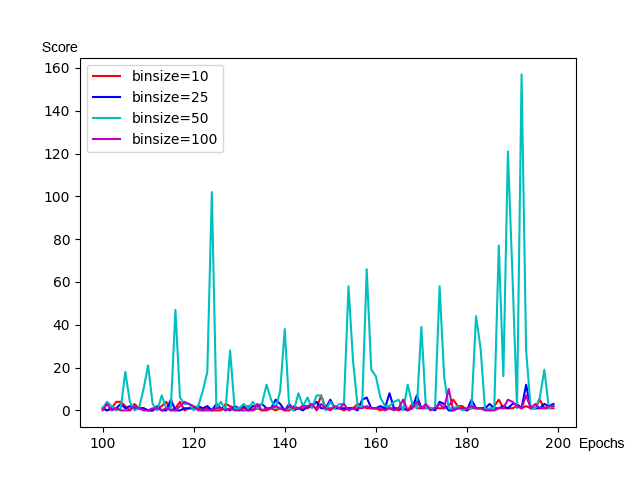
\includegraphics[width=8cm]{binsize.png}
            \caption{Bin Size}
            \label{fig:binsize}
          \end{figure}
          
        \item \textbf{Exploration and Exploitation}\\
        There are 3 parameters related to the exploration-exploitation trade-off:
          \begin{enumerate}
            \item $\alpha_t$: Learning rate. The learning rate determines the impact of the new sample on the current sample. When $\alpha_t$ is large, the learner learns very fast but the result may not converge. So we chose $\alpha_t$ to be inversely proportional to the number of times the state has been visited. Therefore, the learning rate is a generally decreasing function of the number of epochs.
            \item $\gamma$: Future discount rate. Together with learning rate $\alpha$, it affects the impact of future states on current states. The graph in Figure~\ref{fig:Gamma} shows that the optimal future discount rate for our model is around 0.7.
            \begin{figure}[htbp]
            \centering
            \begin{minipage}{.49\textwidth}
            \centering
            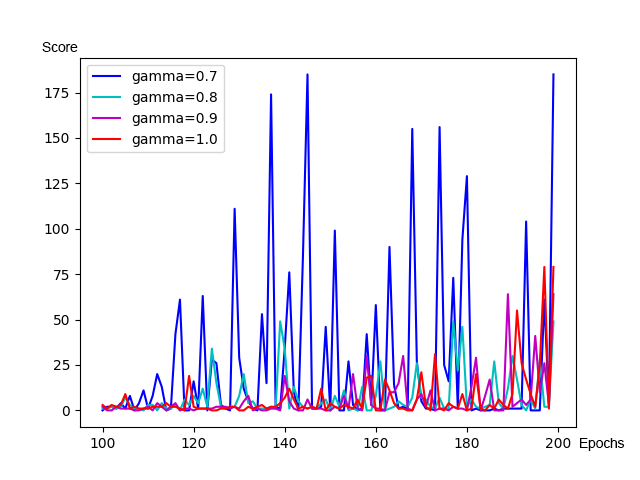
\includegraphics[width=\textwidth]{gamma.png}
            \captionof{figure}{Gamma}
            \label{fig:Gamma}
            \end{minipage}
            \begin{minipage}{.49\textwidth}
            \centering
            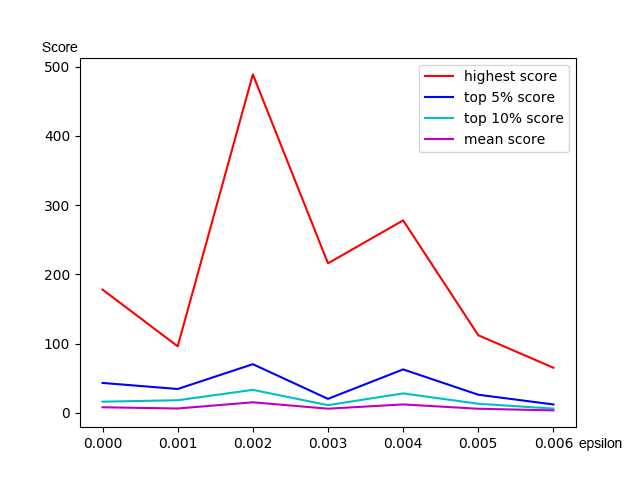
\includegraphics[width=\textwidth]{epsilon.png}
            \captionof{figure}{Epsilon}
            \label{fig:Epsilon}
            \end{minipage}
            \end{figure}
            
            \item $\epsilon$: We adopted the ``$\epsilon$-greedy'' policy for determining the next action. We would like the learner to take more random actions at the beginning so that it could explore more states, and be more consistent with the Q table when we've gathered enough information. Therefore, we also chose $\epsilon$ to be inversely proportional to the number of times the state has been visited. In addition, we want to focus on exploration for the first $80\%$ of the epochs, and on exploitation for the rest. So we use a logistic function for the number of epochs. Let $k_t(s, a)$ denote the number of times $(s, a)$ has been visited at time $t$, then
            \[\epsilon_t = \frac{\epsilon}{k_t(s, a) (1 + e^{(T-0.5t)/T})}  \]
            The results of tuning the parameter $\epsilon$ are shown in Figure~\ref{fig:Epsilon}.
		\end{enumerate}

        \item \textbf{On-policy vs. Off-policy}\\
        Our model-free implementation comprised 2 basic methods: an off-policy approach (Q-learning), where the next action is chosen from the one that maximizes the Q value in the given state, and an on-policy approach (SARSA), where the next action is given by a policy $\pi(s')$. This requires learning a policy $\pi$ in addition to the table of Q values as the game proceeds.
        
        In our SARSA implementation, the policy is initialized to $\pi(s) = 1$ (always jump). Then, under an $\epsilon$-greedy approach, the agent follows the policy $\pi$ with probability $1-\epsilon_t$, and chooses a random action with probability $\epsilon_t$. Finally, the Q values are updated by gradient descent, and the policy is updated as well by the action $a$ that maximizes $Q(s,a)$.
        
      \end{enumerate}


\section{Results}
Table \ref{tab:results} and Figure \ref{fig:Results} show representative results for the 2 main methods we implemented: Q-learning and SARSA.

      \begin{table}[H]
        \centering
        \begin{tabular}{ccccc}
           %\toprule
           Algorithm & Highest & 95\% & 90\% & Median\\
           \midrule
           Q-learning & 2054 & 565.6 & 352.1 & 3.0\\
           SARSA & 610 & 125.0 & 50.2 & 1.0 \\
           %\bottomrule
        \end{tabular}
        \caption{\label{tab:results} Best, 95\%, 90\%, and median scores of Q-learning algorithm}
      \end{table}
      \begin{figure}[H]
        \centering
        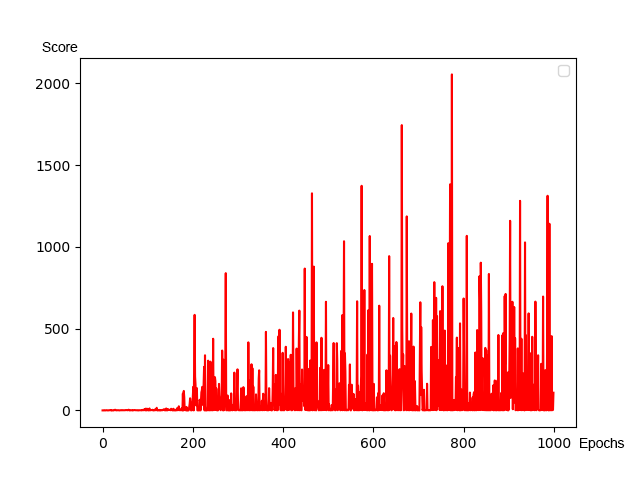
\includegraphics[width=9.5cm]{results.png}
        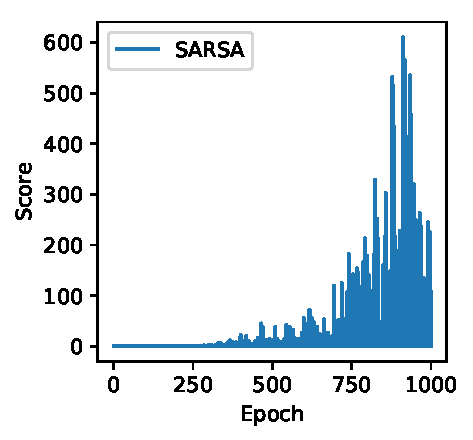
\includegraphics[width=7cm]{results_sarsa.pdf}
        \caption{Final results for algorithms with 1000 epochs: Q-learning (left) and SARSA (right)}
        \label{fig:Results}
      \end{figure}

In general we can see that the Q-learning algorithm yields the better results, and clearly surpasses the minimum results expected for this practical. This would agree with initial expectations, since a well-performing SARSA algorithm requires either a policy that has been optimally constrained from the outset ---for example based on domain knowledge for the particular application---, or an accurate table of Q values that allows a sub-optimal policy to be constantly improved by Policy Iteration.

Another noteworthy result is the different performance of the algorithms under each of the 2 gravity values (1 and 4), where the higher gravity setting consistently yielded better results. More specifically, with the lower gravity in Q-learning, the score was usually under 5 even after a few hundred epochs. On the other hand, the score with the higher gravity was constantly over 100. 

\section{Discussion} 

Our general approach to this problem consisted in implementing model-free Reinforcement Learning, constraining the size of the state space by finding an optimal bin size of 50 pixels to discretize the spatial dimensions of $600 \times 400$ pixels into a maximum of $12 \times 8$ spatial states. By dividing the vertical velocity by 10, we also discretized it into 6 possible velocity states, in addition to the 2 possible gravity states.

In order to balance the exploration/exploitation trade-off, we adopted an $\epsilon$-greedy policy geared towards emphasizing exploration in the initial epochs and exploitation in the final ones. Besides the steps that were taken at random with probability $\epsilon_t$, we implemented a Q-learning (off-policy) method that chose the action that maximized the Q value in the given state, as well as a SARSA (on-policy) method that followed a pre-set policy on every instance. In both cases, the Q table was updated by gradient descent, and in the case of SARSA, the policy was updated as well by Policy Iteration. Further experimentation sought to find optimal values for the learning rate $\alpha_t$, the future discount rate $\gamma$, and the initial exploration probability $\epsilon$.

Our overall results found Q-learning to be the more optimal method for this task, scoring consistently above 100 points and achieving scores of as many as 2000 points, for a gravity setting of 4. For a gravity setting of 1, however, it still proved challenging to learn an accurate Q table within 1000 epochs, most likely as a result of the agent not regularly cycling through as many states in the vertical dimension as it would under stronger gravity.

The off-policy approach of Q-learning makes sense in a setting like the one in this problem, where we have made no prior assumptions on the dynamics of the interaction between the agent and the environment. Without strong assumptions to constrain such interactions into an initial policy, a SARSA algorithm does not perform as well as it could in other circumstances, as seen in the results obtained under that method, which nonetheless also comfortably surpass the requirements for this practical.

\end{document}

